%%%%%%%%%%%%%%%%%%%%%%%%%%%%%%%%%%%%%%%%%%%%%%%%%%%%%%%
%
%                                                       Example IS Template
%
% \documentclass{woosterthesis} must be at the beginning of every IS. Options are the same as
% for the report class with some additional options: abstractonly, acs, alltt, apa, blacklinks, chicago,
% code, colophon, dropcaps, euler, foreignlanguage, gauss, index, kaukecopyright, lshortwooster, maple, mla, palatino, picins,tikz,
% verbatim, wblack, and woostercopyright. The kaukecopyright option will put the arch symbol with the word mark on the
% copyright page. The woosterthesis class is based on the report class. One thing to note is that
% the ``%'' symbol comments out all characters that follow it on the line.
%
%%%%%%%%%%%%%%%%%%%%%%%%%%%%%%%%%%%%%%%%%%%%%%%%%%%%%%%

%%%%%%%%%%%%%%%%%%%%%%%%%%%%%%%%%%%%%%%%%%%%%%%%%%%%%%%
%
% Checked on 8/26/22 and compiles with no fatal errors. Users must have the latest version of the TeXLive software and
% have installed all available packages from CTAN to ensure this thesis class compiles with no fatal errors. Also, you must
% run pdfLaTex, Biber, MakeIndex, padfLaTeX, pdfLaTeX to get all the numbering and references resolved. This is the
% first year the template uses Biber for references.
%
%%%%%%%%%%%%%%%%%%%%%%%%%%%%%%%%%%%%%%%%%%%%%%%%%%%%%%%

%%%%%%%%%%%%%%%%%%%%%%%%%%%%%%%%%%%%%%%%%%%%%%%%%%%%%%%
% use this declaration for a draft  version of your IS
\documentclass[12pt,palatino,code,picins,kaukecopyright,openright,woolshort,dropcaps,verbatim,index,euler]{woosterthesis}
% Note that you can specify the acs option to use the American Chemical Society citation format, apa option to use the American
% Psychological Association citation format, chicago option to use the Chicago citation format, mla option to use the Modern Language
% Association citation format, wblack option for a grayscale Wooster "W" on the cover, and scottie option for a grayscale Scottie Mascot
% on the cover. See exampleis_manual.pdf for an explanation of all the options.
%
%%%%%%%%%%%%%%%%%%%%%%%%%%%%%%%%%%%%%%%%%%%%%%%%%%%%%%%
%
% use this declaration for the print version of your IS
%\documentclass[12pt,palatino,code,picins,blacklinks,kaukecopyright,openright]{woosterthesis} % probably what most students would use
%
%%%%%%%%%%%%%%%%%%%%%%%%%%%%%%%%%%%%%%%%%%%%%%%%%%%%%%%
%
% use this declaration for the PDF version of your IS
%\documentclass[12pt,code,palatino,picins,kaukecopyright,openright]{woosterthesis}
%
%%%%%%%%%%%%%%%%%%%%%%%%%%%%%%%%%%%%%%%%%%%%%%%%%%%%%%%

%%%%%%%%%%%%%%%%%%%%%%%%%%%%%%%%%%%%%%%%%%%%%%%%%%%%%%%
%
%                                                       Load Packages
%
%   To load packages in addition to the ones that are loaded by default, please place your
%   usepackage commands in the packages.tex file in the styles folder.
%
%%%%%%%%%%%%%%%%%%%%%%%%%%%%%%%%%%%%%%%%%%%%%%%%%%%%%%%

%%%%%%%%%%%%%%%%%%%%%%%%%%%%%%%%%%%%%%%%%%%%%%%%%%%%%%%%%%%%%%%%%%%%%%%%%%%%%%%%%%%%%%%%%%%%%%
%
%                                                       Packages
%
% Do not add any other packages without consulting with Dr. Breitenbucher as they may break the functionality of the class.
%
%%%%%%%%%%%%%%%%%%%%%%%%%%%%%%%%%%%%%%%%%%%%%%%%%%%%%%%%%%%%%%%%%%%%%%%%%%%%%%%%%%%%%%%%%%%%%%

\usepackage{lipsum}
\usepackage{pgfplots}

\ifxetex%
	\defaultfontfeatures{Mapping=tex-text,Ligatures=TeX}%
		\setmainfont[Numbers=OldStyle,BoldFont={* Semibold}]{Adobe Garamond Pro}% select the body font other choices would be Baskerville, Optima Regular, Didot, Georgia, Cochin
                      \setmathrm{Adobe Garamond Pro}
                      \setmathfont[Digits,Latin]{Adobe Garamond Pro}
		\setsansfont[Scale=.87,Fractions=On,Numbers=Lining]{Myriad Pro}% select the sans serif font other choices would be Skia, Arial, Helvetica, Helvetica Neue
%		\setmonofont[Scale=.88,Fractions=On]{Prestige Elite Std Bold}% set the mono font other choices would be Courier, Monaco, American Typewriter
	           \setmonofont[Scale=.9]{Courier Std}%
%	    \setromanfont[Fractions=On,Numbers=OldStyle, BoldFont={Warnock Pro Semibold}]{Warnock Pro}%
%	    \setsansfont[Scale=.95,Fractions=On,Numbers=Lining]{Myriad Pro}%
%	    \setmonofont[Scale=.91,Fractions=On]{Courier Std Medium}%
%	    \setmonofont[Scale=.88,Fractions=On]{American Typewriter}%
%		\setmonofont[Scale=.94,Fractions=On]{Prestige Elite Std Bold}
%    		\setromanfont[Fractions=On,Numbers=OldStyle]{Minion Pro}
 %    	\setsansfont[Scale=.9,Fractions=On,Numbers=Lining]{Myriad Pro}
%     	\setmonofont[Scale=.93,Fractions=On]{Courier Std Medium}
%     	\setromanfont[Fractions=On,Numbers=OldStyle]{Minion Pro}
%     	\setsansfont[Scale=.85,Fractions=On,Numbers=Lining]{News Gothic Std}
%    		\setmonofont[Scale=.93,Fractions=On]{Prestige Elite Std}
%		\setromanfont[Fractions=On,Numbers=OldStyle]{Minion Pro}
%		\setsansfont[Scale=.9,Fractions=On,Numbers=Lining]{Bell Gothic Std Bold}
%		\setmonofont[Scale=.95,Fractions=On]{Prestige Elite Std Bold}
\fi


%%%%%%%%%%%%%%%%%%%%%%%%%%%%%%%%%%%%%%%%%%%%%%%%%%%%%%%
%
%                                                       Load Personal commands
%                                                                    
%  There will be certain commands that you use frequently in the thesis. You can give these
%  commands new names which are easier for you to remember. You can also combine several
%  commands into a new command of your own. See The LaTeX Companion or Guide to LaTeX
%  for examples on defining your own commands. These are commands that I defined to cut
%  down on typing. You can enter your commands in the personal.tex file in the styles folder.
%
%%%%%%%%%%%%%%%%%%%%%%%%%%%%%%%%%%%%%%%%%%%%%%%%%%%%%%%

%%%%%%%%%%%%%%%%%%%%%%%%%%%%%%%%%%%%%%%%%%%%%%%%%%%%%%%%%%%%%%%%%%%%%%%%%%%%%%%%%%%%%%%%%%%%%%
%
%                                                       Personal Commands
%                                                                    
% There will be certain commands that you use frequently in the thesis. You can give these
% commands new names which are easier for you to remember. You can also combine several
% commands into a new command of your own. See The LaTeX Companion or Guide to LaTeX for
% examples on defining your own commands. These are commands that I defined to cut down on typing.
%
%%%%%%%%%%%%%%%%%%%%%%%%%%%%%%%%%%%%%%%%%%%%%%%%%%%%%%%%%%%%%%%%%%%%%%%%%%%%%%%%%%%%%%%%%%%%%%

\newcommand{\fl}{\ell}
\newcommand{\lt}{\LaTeX\ }
\newcommand{\msw}{Word\texttrademark\ }
\newcommand{\xt}{\ifthenelse{\boolean{xetex}}{\XeTeX\ }{XeTeX} }
%\newcommand{\Cl}{\ensuremath{\textup{C}_\fl}}
%\newcommand{\bCl}{C$_{\ell}$}
%\newcommand{\Al}{\ensuremath{\textup{A}_\fl}}
%\newcommand{\msum}{{(m_1+\cdots+m_\ell)}}
%\newcommand{\Nsum}{{(N_1+\cdots+N_\ell)}}
%\newcommand{\ysum}{{(y_1+\cdots+y_\ell)}}
%\newcommand{\Nsub}{{N_1+\cdots+N_\ell}}
%\newcommand{\ysub}{{y_1+\cdots+y_\ell}}
%\newcommand{\xsub}{{x_1+\cdots+x_\ell}}
%\newcommand{\ysqsum}{{y_1^2+\cdots +y_{\fl}^2}}
%\newcommand{\msqsum}{{m_1^2+\cdots +m_{\fl}^2}}
%\newcommand{\ratio}{\left(\frac{\beta}{\alpha}\right)}
%\newcommand{\LT}{\ensuremath{\LaTeX{}}}

%%%%%%%%%%%%%%%%%%%%%%%%%%%%%%%%%%%%%%%%%%%%%%%%%%%%%%%%%%%%%%%%%%%%%%%%%%%%%%%%%%%%%%%%%%%%%%
% These commands have one argument and are entered as \commandname{argument}.
%%%%%%%%%%%%%%%%%%%%%%%%%%%%%%%%%%%%%%%%%%%%%%%%%%%%%%%%%%%%%%%%%%%%%%%%%%%%%%%%%%%%%%%%%%%%%%

%\newcommand{\bd}[1]{\textbf{#1}}
\newcommand{\mbd}[1]{{\mathbf{#1}}}
%\newcommand{\abs}[1]{\vert{#1}\vert}
\newcommand{\bvec}[1]{{\mbd{#1}}}
%\newcommand{\lvec}[1]{\abs{\bvec{#1}}}
%\newcommand{\nesmallprod}[1]{\prod_{\substack{#1=1\\
%#1\neq p}}^{\fl}}
%\newcommand{\esec}[1]{e_{2}({#1}_1,\ldots ,{#1}_\fl)}
%\newcommand{\smallprod}[1]{\prod_{#1=1}^{\fl}}
%\newcommand{\incsum}[1]{{#1}_2+2{#1}_3+\cdots +(\fl -1){#1}_\fl}
%\newcommand{\binomsum}[1]{\binom{{#1}_1}{2}+\cdots +\binom{{#1}_\fl}{2}}
%\newcommand{\imultsum}[1]{\multsum{{#1}_k\ge 0}{k=1,\ldots ,\fl}}
%\newcommand{\diagsum}[1]{\sum _{\substack{{#1}_k\ge 0\\
%k=1, \ldots ,\fl\\
%\lvec{#1}=m}}}
%\newcommand{\Mb}[1][\fl]{\ensuremath{\textup{\bd{M}}_b^{(#1)}}}
%\newcommand{\HLV}[1]{\ensuremath{\textup{\bd{H}}_{#1}}}
%\newcommand{\Rq}[1][p]{\ensuremath{\textup{R}_q^{(#1)}}}
\newcommand{\degree}[1]{\ensuremath{#1^{\circ}}}
\newcommand{\ip}[1]{\texttt{#1}\index{packages!#1}}
\newcommand{\ic}[1]{\texttt{$\backslash$#1}\index{commands!#1}}
\newcommand{\ie}[1]{#1\index{#1}}

%%%%%%%%%%%%%%%%%%%%%%%%%%%%%%%%%%%%%%%%%%%%%%%%%%%%%%%%%%%%%%%%%%%%%%%%%%%%%%%%%%%%%%%%%%%%%%
% These commands have 2 or more arguments some with default values for the first argument. You
% can learn a lot about constructing complicated equations by studying the commands in this %section.
%%%%%%%%%%%%%%%%%%%%%%%%%%%%%%%%%%%%%%%%%%%%%%%%%%%%%%%%%%%%%%%%%%%%%%%%%%%%%%%%%%%%%%%%%%%%%%

%\newcommand{\qbinom}[2]{\ensuremath{\left[{#1}\atop{#2}\right]_q}}
%\newcommand{\sqprod}[2]{\prod_{#1,#2=1}^{\fl}}
%\newcommand{\triprod}[2]{\prod_{1\le #1<#2\le \fl}}
%\newcommand{\nesqprod}[2]{\prod_{\substack{#1,#2=1\\
%#1,#2\neq p}}^{\fl}}
%\newcommand{\netriprod}[2]{\prod_{\substack{1\le #1<#2\le \fl\\
%#1,#2\neq p}}}
\newcommand{\qrfac}[3][\ ]{\left({#2}\right)_{#3}^{#1}}
%\newcommand{\multsum}[2]{\sum_{\substack{{#1}\\
%\\
%{#2}}}}
%\newcommand{\fmultsum}[2][N]{\multsum{0\le {{#2}_k}\le {{#1}_k}}{k=1,\ldots ,\fl}}
%\newcommand{\pq}[2]{\ _{#1}\varphi_{#2}}
%\newcommand{\mess}[2][y_k]{\frac{\qrfac{\alpha x_k}{#2}\qrfac{qx_k\beta^{-1}}{#2}}{\qrfac{\beta x_k}{#1}
%\qrfac{qx_k\alpha^{-1}}{#1}}}
%\newcommand{\MG}[7][\fl]{\ensuremath{\left[\textup{MG}\right]_{#2}^{(#1)}{#3}q;{#4};{#5}^{#6}{#7}}}

%%%%%%%%%%%%%%%%%%%%%%%%%%%%%%%%%%%%%%%%%%%%%%%%%%%%%%%%%%%%%%%%%%%%%%%%%%%%%%%%%%%%%%%%%%%%%%
% These commands define new environments
%%%%%%%%%%%%%%%%%%%%%%%%%%%%%%%%%%%%%%%%%%%%%%%%%%%%%%%%%%%%%%%%%%%%%%%%%%%%%%%%%%%%%%%%%%%%%%

\newcounter{unnumft}
\setcounter{unnumft}{0}
\newenvironment{unnumft}[2]{\renewcommand{\thefootnote}{}\footnote{#1}\footnote{#2}} {\addtocounter{footnote}{-2}}
\newenvironment{wooexample}{\small
\begin{singlespace}
\begin{example}}{\end{example}
\end{singlespace}}

\graphicspath{{./figures/}}% for setting where to look for figures
%\citestyle{wooster}% change the style of citations. Math and CS people should leave this alone.

%%%%%%%%%%%%%%%%%%%%%%%%%%%%%%%%%%%%%%%%%%%%%%%%%%%%%%%%%%%%%%%%%%%%%%%%%%%%%%%%%%%%%%
% Modify the formatting of the back references
%%%%%%%%%%%%%%%%%%%%%%%%%%%%%%%%%%%%%%%%%%%%%%%%%%%%%%%%%%%%%%%%%%%%%%%%%%%%%%%%%%%%%%
\DefineBibliographyStrings{english}{%
	backrefpage  = {page }, % for single page number
	backrefpages = {pages } % for multiple page numbers
}






%%%%%%%%%%%%%%%%%%%%%%%%%%%%%%%%%%%%%%%%%%%%%%%%%%%%%%%
%
%                                                       Load Theorem formatting information
%
%  If you need to define an new theorem style or want to see what theorem like environments 
%  are available please look at the theorems.tex file in the styles folder.
%
%%%%%%%%%%%%%%%%%%%%%%%%%%%%%%%%%%%%%%%%%%%%%%%%%%%%%%%

%%%%%%%%%%%%%%%%%%%%%%%%%%%%%%%%%%%%%%%%%%%%%%%%%%%%%%%%%%%%%%%%%%%%%%%%%%%%%%%%%%%%%%%%%%%%%%
%
% This is where one would tell \LaTeX{} how to format Theorems, Definitions, etc. and also
% indicate the environment names. You need the amsthm package (loaded in the woosterthesis %class) in order for these commands to work.
%
%%%%%%%%%%%%%%%%%%%%%%%%%%%%%%%%%%%%%%%%%%%%%%%%%%%%%%%%%%%%%%%%%%%%%%%%%%%%%%%%%%%%%%%%%%%%%%

% an example of defining your own theoremstyle
%\newtheoremstyle{break}% name
%  {\topsep}%      Space above
%  {\topsep}%      Space below
%  {\itshape}%         Body font
%  {}%         Indent amount (empty = no indent, \parindent = para indent)
%  {\bfseries}% Thm head font
%  {.}%        Punctuation after thm head
%  {\newline}%     Space after thm head: " " = normal interword space;
%        %       \newline = linebreak
%  {}%         Thm head spec (can be left empty, meaning `normal')
\newtheoremstyle{scthm}{\topsep}{\topsep}{\itshape}{}{\bfseries\scshape}{}{ }{}% small cap font for the heading
\newtheoremstyle{itdefn}{\topsep}{\topsep}{\itshape}{}{\bfseries}{.}{ }{}% italic definitions
\newtheoremstyle{scdefn}{\topsep}{\topsep}{\itshape}{}{}{}{ }{\thmname{\textbf{#1}}\thmnumber{ \textbf{#2}}\thmnote{ \scshape #3:}}% small cap headings and italic text.

\theoremstyle{break}% this theoremstyle will put the text of the theorem on a new line.
\newtheorem{thm}{Theorem}[chapter]%number theorems within chapters 
%\newtheorem{cor}[thm]{Corollary}%by using [thm] we are numbering these environments with the theorems.
\newtheorem{cor}{Corollary}[chapter]%number corollaries within chapters .
%\newtheorem{lem}[thm]{Lemma}
\newtheorem{lem}{Lemma}[chapter]
%\newtheorem{prop}[thm]{Proposition}
\newtheorem{prop}{Proposition}[chapter]

\theoremstyle{scdefn}
%\newtheorem{defn}[thm]{Definition}
\newtheorem{defn}{Definition}[chapter]
\theoremstyle{remark}
%\newtheorem{rem}[thm]{Remark}
\newtheorem{rem}{Remark}[chapter]
\renewcommand{\therem}{}
%\newtheorem{ex}[thm]{Example}
\newtheorem{ex}{Example}[chapter]

\theoremstyle{plain}
%\newtheorem{note}[thm]{Notation}
\newtheorem{note}{Notation}[chapter]
\renewcommand{\thenote}{}
%\newtheorem{nts}[thm]{Note to self}%use to remind yourself of things yet to do
\newtheorem{nts}{Note to self}[chapter]
\renewcommand{\thents}{}
%\newtheorem{terminology}[thm]{Terminology}
\newtheorem{terminology}{Terminology}[chapter]
\renewcommand{\theterminology}{}

\theoremstyle{itdefn}
\newtheorem{bdefn}{Definition}[chapter]
\newsavebox{\fmbox} 
\newenvironment{boxeddefn}[2] 
{\begin{lrbox}{\fmbox}\begin{minipage}{0.9 \linewidth }\begin{singlespace}\begin{bdefn}[{#1}]\label{#2}\vspace{0.2cm}} 
{\end{bdefn}\end{singlespace}\end{minipage}\end{lrbox}\fbox{\usebox{\fmbox}}}

\setcounter{secnumdepth}{5}% controls the numbering of sections
\setcounter{tocdepth}{6}% controls the number of levels in the Contents

%%%%%%%%%%%%%%%%%%%%%%%%%%%%%%%%%%%%%%%%%%%%%%%%%%%%%%%
%
%  This is where one enters their bibilography file name.
%
%%%%%%%%%%%%%%%%%%%%%%%%%%%%%%%%%%%%%%%%%%%%%%%%%%%%%%%

\addbibresource{references.bib}

%%%%%%%%%%%%%%%%%%%%%%%%%%%%%%%%%%%%%%%%%%%%%%%%%%%%%%%
%
%  This is where one enters the information about the thesis.
%
%%%%%%%%%%%%%%%%%%%%%%%%%%%%%%%%%%%%%%%%%%%%%%%%%%%%%%%

\title{Something something reverb}
\thesistype{Independent Study Thesis} % you should make this Independent Study Thesis
\author{William Sieber}
%\presentdegrees{Ph.D.} % you should comment this line
\degreetoobtain{Bachelor of Arts in Computer Science and Music}
\presentschool{The College of Wooster}
\academicprogram{Department of Mathematical \& Computational Sciences and Department of Music}
\gradyear{2024}
\advisor{Daniel Palmer (Computer Science)}
\secondadvisor{Greg Slawson (Music)}
%\reader{Reader}
\copyrighted   
%\copyrightdate{}                  
\makeindex % comment this line if you do not have an index

%%%%%%%%%%%%%%%%%%%%%%%%%%%%%%%%%%%%%%%%%%%%%%%%%%%%%%%
%
%  This is where the commands for the document begin. All \LaTeX{} documents must have a
%  \begin{document} text .... \end{document} structure.
%
%%%%%%%%%%%%%%%%%%%%%%%%%%%%%%%%%%%%%%%%%%%%%%%%%%%%%%%

\begin{document}

%%%%%%%%%%%%%%%%%%%%%%%%%%%%%%%%%%%%%%%%%%%%%%%%%%%%%%%
%
%  The front matter includes acknowledgments, dedications, vitas, list of tables, list of figures,
%  copyright, abstract, title page, and contents.
%
%%%%%%%%%%%%%%%%%%%%%%%%%%%%%%%%%%%%%%%%%%%%%%%%%%%%%%%

\frontmatter
\maketitle
%\ClearShipoutPicture
\clearpage\thispagestyle{empty}\null\clearpage
\disscopyright 

%%%%%%%%%%%%%%%%%%%%%%%%%%%%%%%%%%%%%%%%%%%%%%%%%%%%%%%
%                                                                                       
%                                                       Abstract						
%                                                                                       
%%%%%%%%%%%%%%%%%%%%%%%%%%%%%%%%%%%%%%%%%%%%%%%%%%%%%%%

\begin{abstract}
[abstract]
%Artificial reverberation is a method of adding ``echo'' to a particular sound to achieve a desired effect. In doing so, a signal with a short response time can make sound as if it is played in a bathroom, concert hall, or cathedral. Common C++ implementations of this effect usually fall under two different categories: \textit{Feedback Delay Networks} (FDNs) or \textit{Convolution Algorithms}. The former creates this effect via a number of delay lines in parallel, resulting in a reverberated sound provided a sufficiently high echo density is created. The latter uses the frequency response of an acoustic space to generate a realistic sounding reverberation, which is added to the input signal. This thesis studies the practical and sonic differences between these algorithms and their implementations. The final program will allow producers to use either one of these algorithms independently in the Digital Audio Workstation of their choice.
\end{abstract}

%%%%%%%%%%%%%%%%%%%%%%%%%%%%%%%%%%%%%%%%%%%%%%%%%%%%%%%
%                                                                                       
%                                                       Dedications					
%                                                                                       
%%%%%%%%%%%%%%%%%%%%%%%%%%%%%%%%%%%%%%%%%%%%%%%%%%%%%%%

%\dedication{This work is dedicated to the future generations of Wooster students.}


%%%%%%%%%%%%%%%%%%%%%%%%%%%%%%%%%%%%%%%%%%%%%%%%%%%%%%%
%                                                                                       
%                                                       Acknowledgments					
%                                                                                       
%%%%%%%%%%%%%%%%%%%%%%%%%%%%%%%%%%%%%%%%%%%%%%%%%%%%%%%

\begin{acknowl}  
[acknowledgments]
\end{acknowl}

%%%%%%%%%%%%%%%%%%%%%%%%%%%%%%%%%%%%%%%%%%%%%%%%%%%%%%%
%                                                                                       
%                                                       Vita					
%                                                                                       
%%%%%%%%%%%%%%%%%%%%%%%%%%%%%%%%%%%%%%%%%%%%%%%%%%%%%%%

%\begin{vita}
% You talk about yourself and how you got to where you are now. There is a structured form for the Vita that can be used if you want, but I don't encourage it.

%%%%%%%%%%%%%%%%%%%%%%%%%%%%%%%%%%%%%%%%%%%%%%%%%%%%%%%
%
%  The list below is for a thesis that requires a more structured Vita such as a masters or Ph.D.
%
%%%%%%%%%%%%%%%%%%%%%%%%%%%%%%%%%%%%%%%%%%%%%%%%%%%%%%%

%\begin{datelist}
%\item[August 11, 1990]Chosen to present an undergraduate paper at the 75th meeting of the MAA, Columbus, Ohio
%\item[August 1990--August 1991]President Wooster Student Chapter of the MAA, The College of Wooster, Wooster, Ohio
%\item[August 1991--May 1992]Secretary Wooster Student Chapter of the MAA, The College of Wooster, Wooster, Ohio
%\item[1992]\emph{Phi Beta Kappa} (on junior standing), The College of Wooster, Wooster, Ohio
%\item[1992]Elizabeth Sidwell Wagner Prize in Mathematics, The College of Wooster
%\item[1992]William H. Wilson Prize in Mathematics, The College of Wooster
%\item[May 11, 1992]B.A., Mathematics, The College of Wooster
%\item[1997]Finalist for Graduate Teaching Award, The Ohio State University, Columbus, Ohio
%\item[June 21-25, 1998]Participant in the AMS-IMS-SIAM Summer Research Conferences: q-Series, Combinatorics, and Computer Algebra, Mt. Holyoke, Massachusetts
%\item[October 1998--October 1999]Graduate student representative to The Ohio State University Department of Mathematics Graduate Studies Committee, Columbus, Ohio
%\item[January 1999]q-series seminar address, The Ohio State University, Columbus, Ohio
%\item[2000]Finalist for Departmental Teaching Award, The Ohio State University, Columbus, Ohio
%\item[2000]Nominated for Graduate Teaching Award, The Ohio State University, Columbus, Ohio
%\item[April 2000]Invited colloquium talk at The College of Wooster, Wooster, Ohio
%\item[1992-- present]Graduate Teaching and Research Associate, The Ohio State University
%\end{datelist}
%
%%%This is for any publications you might have.%%%%%

%\end{vita}

%%%%%%%%%%%%%%%%%%%%%%%%%%%%%%%%%%%%%%%%%%%%%%%%%%%%%%%
%
%  We now create the contents page and if necessary the list of figures and list of tables.
%
%%%%%%%%%%%%%%%%%%%%%%%%%%%%%%%%%%%%%%%%%%%%%%%%%%%%%%%


\cleardoublepage
\phantomsection
\addcontentsline{toc}{chapter}{Contents}

\tableofcontents
\listoffigures %Use if you have a list of figures.
\listoftables%Use if you have a list of tables.
\lstlistoflistings% Use if you are using the code option

%%%%%%%%%%%%%%%%%%%%%%%%%%%%%%%%%%%%%%%%%%%%%%%%%%%%%%%

%%!TEX root = ../username.tex
\chapter*{Preface}\label{pref}
\addcontentsline{toc}{chapter}{Preface}

Here is how I plan on introducing you to \LaTeX. The Introduction gives some reasons for why one might find \lt superior to MS Word\texttrademark. Chapter \ref{text} will demonstrate how one starts typesetting a document and works with text in \LaTeX. Chapter \ref{graphics} discusses the creation of tables and how one puts figures into a thesis. Chapter \ref{bibind} talks about creating a bibliography/references section and an index. There are three Appendices which discuss typesetting mathematics and computer program code. The Afterword will discuss some of the particulars of how a \lt document gets processed and what packages the \texttt{woosterthesis} class uses and are assumed to be available on your system.
 % most theses do not have a preface so this should be commented

%%%%%%%%%%%%%%%%%%%%%%%%%%%%%%%%%%%%%%%%%%%%%%%%%%%%%%%
\mainmatter

%%%%%%%%%%%%%%%%%%%%%%%%%%%%%%%%%%%%%%%%%%%%%%%%%%%%%%%
%
%                                                       Thesis Chapters
%
% This is where the main text of the thesis goes. I have written this template assuming that
% each chapter is a separate file. You do not have to do this but it makes things easier to find
% for editing. You can use the sample chapters to help you figure out how to type things into
% your thesis. To include a chapter just use the \include{chaptername} command. Chapters are
% included in the order listed.
%
%%%%%%%%%%%%%%%%%%%%%%%%%%%%%%%%%%%%%%%%%%%%%%%%%%%%%%%

%!TEX root = ../username.tex
\chapter{Introduction}\label{intro}
%holy jank but i figured it out
\hspace*{-0.132cm}Meaningful songs take the listener on a journey. Regardless of genre, music has the ability to connect people together of a wide variety of backgrounds and experiences. In one way, a composer chooses different notes in a piece to follow particular harmonic and melodic conventions. Meeting these conventions and subverting them in interesting ways is part of what makes music, music. In another way, much like a song's chord progression, the timbre of a sound itself can create greater depth and immersion in one's production to help bring the listener from point ``A'' to point ``B''. Several tools are at a producer's disposal to modify the color and shape of a particular sound in real time. For example, distortion can be added to a guitar, or delay can be added to a singer's vocals. Reverb is another such essential tool at the producer's disposal used in music production today.

The study of artificial reverberation goes back over a hundred years. During this time, the methods used to artificially reverberate sound has shifted from ad hoc methods to carefully crafted tools and programs. Today, the majority of programs are created for use under specific host applications. By easily handling input and output of other programs which manipulate a given signal, one can perform complex sound design by utilizing a combination of several programs in series.

What follows is a study into the development and execution of artificial reverberation in C++. To better understand how reverberation is used in the context of music production, we will begin with a historical view of this tool. Next, we will look at the programs and software that producers use to create music today, and in what ways they use reverberation. Specifically, this will include discussion of Digital Audio Workstations and their associated programs. After, we will consider the digital signal processing theory required to create these tools. This will include how to represent sound in a digital manner and in what ways the computer processes this sound. Finally, we will discuss various methods of persisting sound with a short impulse. Someone inexperienced in this topic should not only gain an understanding in how artificial reverberators are made, but also be able to implement one themselves.

%!TEX root = ../username.tex
\chapter{Background}
\hspace*{-0.155cm}This chapter will provide the backgorund information necessary to understand what artificial reverberators are, why their use is important, and the different ways they are used by musicians today. It will begin with a broad definition of ``reverberation'' and discuss how sound persists in real-world spaces. After, it will discuss various methods of reverberating sound. Lastly, it will discuss how reverb is used today.

\section{What is Reverb?}
Imagine yourself speaking in a large concert hall. The audience does not only your your voice; they hear the combination of both your voice and the reflections of your voice off the walls and stage you are speaking on. In the right context, they serve both an artistic and practical purpose by enhancing the qualities of the sound being made on stage. In a broad sense, reverb can be defined as ``an ambient space in the perception of the listener'' \cite{dattorro1997effect}. This can take many different forms. Sound waves bouncing off the walls of a room, sound waves traveling through springs, sound waves traveling through a computer program - these are a few such ways in which a perceived ambient space can be created. It provides a texture that is considered ``wet'' and washes out the sound of an otherwise clear tone. In small amounts, it can be tasteful and enhance the timbre of an instrument. In large amounts, it can overpower the initial tone and can disrupt other elements of the music, such as rhythm \cite{blesser2007spaces}.

Consider an instrument with a short impulse response:

\begin{figure}[h] % [h] used to prevent {figure} from doing weird positioning
	\begin{center}
		\fbox{
		\begin{tikzpicture}
			\begin{axis} [
				axis x line = middle, % The x axis should go through the origin
				no markers,
				xlabel = \(t\),
				ylabel = {\(f(t)\)},
				height = 5cm,
				width = 12cm,
				xmin=0,
				xtick distance=0.2,
				]
				\addplot [
					red,
					thick
				] table [x=step,y=wav,col sep=comma] {test.csv};
			\end{axis}
		\end{tikzpicture}
		}
		\caption{A waveform of a snare drum.}
	\end{center}
\end{figure}

By adding reverb, this same instrument can sound as if it were performed in a large room:

\begin{figure}[h] % [h] used to prevent {figure} from doing weird positioning
	\begin{center}
		\fbox{
		\begin{tikzpicture}
			\begin{axis} [
				axis x line = middle, % The x axis should go through the origin
				no markers,
				xlabel = \(t\),
				ylabel = {\(f(t)\)},
				height = 5cm,
				width = 12cm,
				xtick distance=1,
				]
				\addplot [
					red,
					thick
				] table [x=step,y=wav,col sep=comma] {test2.csv};
			\end{axis}
		\end{tikzpicture}
		}
		\caption{A waveform of a snare drum with reverberation.}
	\end{center}
\end{figure} %fix to compress waveform to -1 and 1

Prior to the early 1960s, \textit{artificial reverberators} were physical devices - that is, something that took input from an electromechanical transducer and manipulated the sound using a variety of physical methods. Some such devices used metal plates, springs, and oil canisters - each providing their own unique sound and characteristics \cite{FiftyYears}. In some cases, these sounds were desirable and used for their specific timbral qualities. Some programs today aim to replicate the sound of these early devices. Many, however, prefer to mimic the sound that would be expected of a large hall, without any of the uniqueness of other methods. In 1961, M. R. Schroeder introduced a number of methods to digitally recreate reverb without additional color \cite{schroeder1961natural}. These same algorithms are used in several programs today.

\section{Historical Developments}
Prior to purely electronic means, there existed several methods of persisting sound with a short impulse. One such method is simply using a physical room. \textit{Echo chambers} are rooms constructed lacking parallel surfaces to effectively reverberate a sound \cite{FiftyYears}. They contain a speaker and a microphone to record the input signal once it has been reverberated, which is then mixed back with the original signal. Their primary benefit come from the method itself - using a real room will produce a sound that is nearly indistinguishable to an otherwise reverberant hall. While echo chambers continue to exist today, their use is limited to those who have the infrastructure to build and maintain such rooms. They are most commonly found in recording studios, or otherwise special music production spaces. For individual devices, there are other methods of reverberating sound that are more convenient and cost effective.

\textit{Spring Reverberators} are another method. Their primary benefit is that they were compact - a much more convenient solution than an echo chamber. They were invented by Laurens Hammond after he patented the invention in 1941 \cite{laurens1941electrical}. In said patent, he describes a device in which sound traveling through a wire is sent through springs reinforced to the device, creating a reverberant sound. This reverberated signal is then sent back to be mixed with the original. Their small footprint allowed for their inclusion in devices such as synthesizers, a diagram of which can be seen below in Figure 2.3.

\begin{figure}[h] % [h] used to prevent {figure} from doing weird positioning
	\begin{center}
		\fbox{
		\includegraphics[width=16cm]{figures/elect.png}
		}
		\caption{A model of a Spring Reverberator \cite{devoe1977electronmusic}.}
	\end{center}
\end{figure}

Electromechanical devices such as these are not perfect, however. Their sound may provide an approximation of what might be heard in an echo chamber, but is not a perfect replication of the original. \textit{Plate reverberators} fall under a similar vein - sound travels through the plate and is mixed back with the original ``dry'' signal.

\section{How is Reverb Used Today?}
Nowadays, nearly every song one hears on the radio utilizes some kind of music application which allows one to record, edit, and manipulate several audio sources and recordings. Such applications are known as \textit{Digital Audio Workstations} (DAWs). By allowing the producer to manipulate recordings in real time, they can quickly and efficiently create the music that one hears today. DAWs accomplish this by providing tools to record the notes or sounds of instruments through various means. For example, virtual instruments stored on the producer's PC can be performed by a MIDI keyboard conneced to the DAW. These virtual instruments are known as \textit{plugins}, a type of application that runs under a DAW.

Plugins are generally broken into two distinct categories: \textit{generator plugins} and \textit{effect plugins}. Their difference is self-explanatory; generator plugins sample or synthesize a sound within the application, while effect plugins manipulate a given input. For the purposes of this thesis, focus will be placed on the development of \textit{effect plugins}. The producer can apply several of these effect plugins to a source sound in series. Effect plugins can range from distortion to chorus to arpeggiators, but they all operate using the same principle - take a signal as input, perform some type of operation to it, and return the processed signal. Reverb is one type of effect plugin that is often used in DAWs; an example of one such DAW can be seen in Figure 2.4.

\begin{figure}[h] % [h] used to prevent {figure} from doing weird positioning
	\begin{center}
		\fbox{
		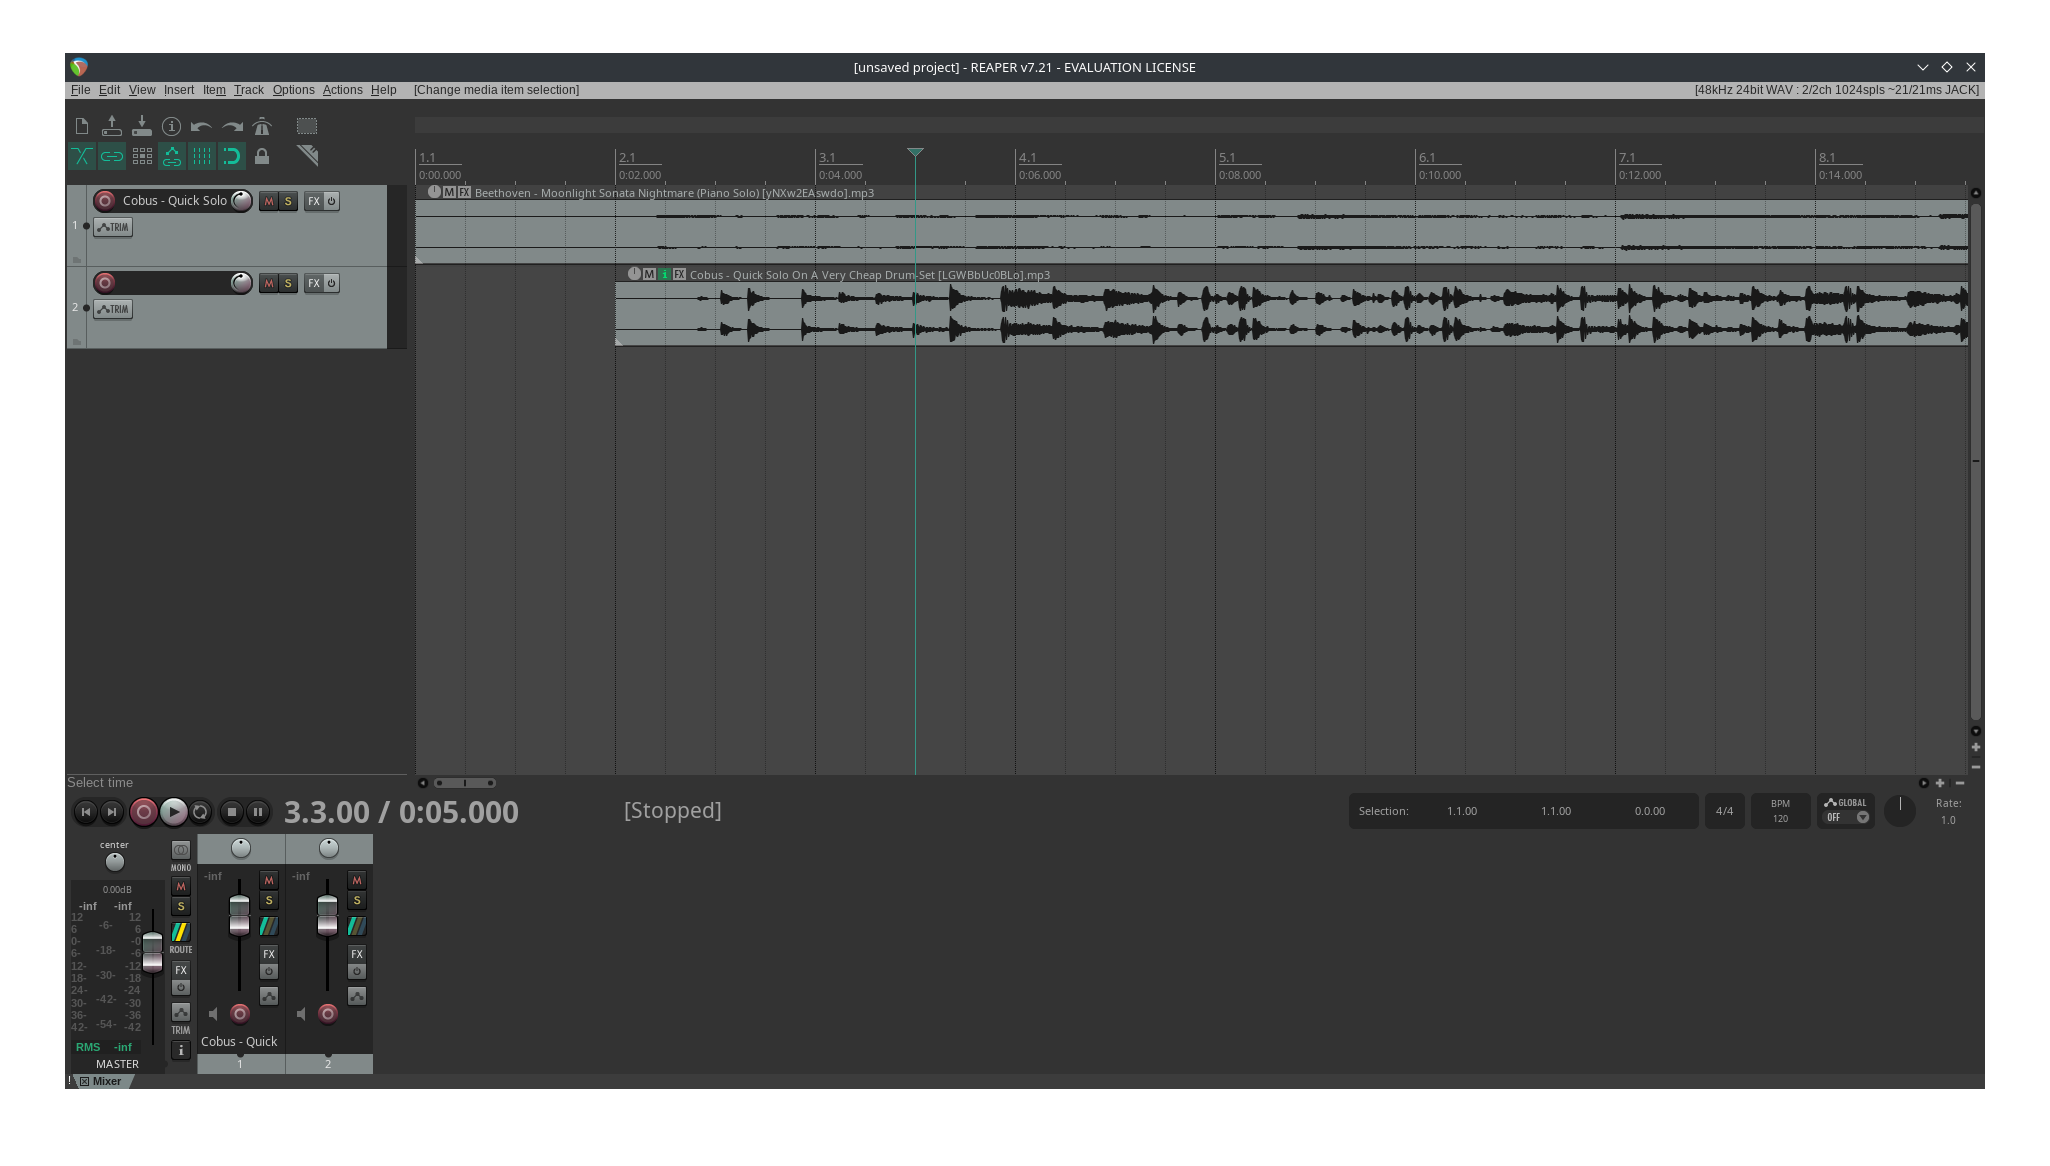
\includegraphics[width=16cm]{figures/DAW.png}
		}
		\caption{A screenshot of Reaper - a Digital Audio Workstation.}
	\end{center}
\end{figure}

While DAWs can differ in look and feel, they are generally broken into three separate areas:

\begin{itemize}
  \item The timeline: located in the middle, this contains each waveform and allows the producer to arrange how and when tracks are played.
  \item The track control panel: located on the left, this allows the producer to add and remove different tracks in a project.
  \item The mixer control panel: located on the bottom, this allows the producer to adjust the volume of individual tracks and add effects.
\end{itemize}

These three sections are included in nearly every DAW available today. In practice, they allow producers to change when sounds occur and their volume by an exact amount. Through these tools, producers are able to create nearly any sound they can imagine; they can take parts of other songs and deconstruct them into something new; they can create an effect chain so complex that they turn a simple snare drum into something unrecognizable. Their only limit is their creativity.

%!TEX root = ../username.tex
\chapter{Realtime Audio Programming}

\section{Obstacles to Overcome}
\section{The VST Software Development Kit}

%!TEX root = ../username.tex
\chapter{Artificial Reverberation Design}
\hspace*{-0.15cm}This chapter will begin with a brief overview of digital signal processing to understand artificial reverberation algorithms. After, various methods of reverberation will be explored; specifically going into detail how they work and their corresponding signal flow graphs.

\section{Filters \& Signal Flow Graphs}
Thus far, signals have been represented as a function with respect to time. This is not the only manner in which one can visualize audio, however - by computing the \textit{Fourier Transform} of a function, it can be graphed as a function with respect to \textit{frequency}, as opposed to time. At a high level, the Fourier Transform deconstructs a signal to its sinusoids; this was discussed in Chapter 3. However, to compute the Fourier Transform, the previously discussed mathematical representation of sound will need to be reevaluated.

Phase shifted sinusoids are ambiguous as to how they can be represented mathematically. That is, the same sinusoid can be represented as a function of sine \textit{or} cosine. To perform calculations useful to the programmer, one needs a representation of a sinusoidal wave that removes this ambiguity. The \textit{complex sinusoid} does exactly that by encapsulating both functions under the complex plane \cite{pirkle2019designing}:

\begin{defn}[Definition of a complex sinusoid]\label{def-complex}
	\begin{equation}\label{eq-complex)}
	e^{j\omega t} = cos(\omega t) + j sin(\omega t)
\end{equation}\end{defn}

where $\omega$ is radians, $t$ is time, and $j$ is $ \sqrt{-1}$. With this definition, the Fourier Transform $X(\omega)$ may be calculated from a signal $x(t)$.

\begin{defn}[Definition of the Fourier Transform \cite{MDFTWEB07}]\label{def-Cont-FT}
	\begin{equation}\label{eq-Cont-FT)}
	X(\omega) = \int_{-\infty}^\infty x(t)e^{-j\omega t}dt, \quad \omega \in (-\infty, \infty)
\end{equation}\end{defn}

In a digital setting, this process is computed via the summation of samples from a given input buffer:

\begin{defn}[Definition of the Discrete Fourier Transform \cite{MDFTWEB07}]\label{def-disCont-FT}
	\begin{equation}\label{eq-disCont-FT)}
	X(\omega_k) = \sum_{n=0}^{N-1} x(t_n)e^{-j\omega_k t_n}, \quad k = 0,1,2,..., N - 1
\end{equation}\end{defn}

Revisiting the Nyquist-Shannon Sampling Theorem, one may graph the bandlimited signal $F_{max}$ and Nyquist Rate $F_s$ with respect to frequency using a DFT. Such an example can be seen below:

\begin{figure}[h] % [h] used to prevent {figure} from doing weird positioning
	\begin{center}
		\fbox{
		\begin{tikzpicture}
            \begin{axis} [
			axis x line = middle, % The x axis should go through the origin
			axis y line = middle,
			xmin = -7,
			xmax = 7,
			ymin = -1.5,
			ymax = 7,
			xlabel = \(f\),
			ylabel = {\(X(f)\)},
			height = 7cm,
			width = 13cm,
			xtick distance=6,
			ytick distance=-10,
			xticklabel = \empty
			]
			\addplot[very thick, red][domain=-3:-2]{+0.8*x^3+7.2*x^2+22.5*x^1+24.3*x^0};
			\addplot[very thick, red][domain=-2:-1]{+-2.4*x^3+-12*x^2+-15.9*x^1+-1.3*x^0};
			\addplot[very thick, red][domain=-1:0]{+2.9*x^3+3.9*x^2+8.608e-62*x^1+4*x^0};
			\addplot[very thick, red][domain=0:1]{+-2.9*x^3+3.9*x^2+8.608e-62*x^1+4*x^0};
			\addplot[very thick, red][domain=1:2]{+2.4*x^3+-12*x^2+15.9*x^1+-1.3*x^0};
			\addplot[very thick, red][domain=2:3]{+-0.8*x^3+7.2*x^2+-22.5*x^1+24.3*x^0};
			\node[draw] at (1000, 70) {$F_{max}$};
			\node[draw] at (400, 70) {$F_{max}$};
			\node[draw] at (1300, 70) {$F_{s}$};
			\node[draw] at (100, 70) {$F_{s}$};
			\end{axis}
		\end{tikzpicture}
		}
		\caption{An example of a Fourier Transform taken from a bandlimited function.}
	\end{center}
\end{figure}

It is worth reiterating - with this representation, $f$ represents frequency on the x-axis, and $X(f)$ represents the \textit{amplitude} of frequencies. It begs the question - how does this relate to reverberation, exactly?

Recall the way a digital audio workstation functions. Generated sound is sent through various mixer channels to be modified before combining in the master channel. While various effects are available to manipulate sound in the mixer, exactly \textit{how} they work is behind closed doors. Musicians may be familiar with tools such as ``lowpass filters'' and ``highpass filters''. Audio engineers expand what exactly a ``filter'' is to include \textit{all} types of different effects - or black boxes, rather.

With this in mind, a \textit{filter} can be defined as a medium through which a signal enters as an input and exits as an output \cite{FILTERS07}. It is a type of \textit{black box system} whose inner workings modify the sound in some way; it is inclusive of any type of effect one can think of. By extension, a \textit{digital filter} is a type of filter that operates on digital signals in the form of a computation. This computation can take the form of an equation, or a snippet of code in a computer.

Take the following filter, for example:

\begin{figure}[h] % [h] used to prevent {figure} from doing weird positioning
	\begin{center}
		\fbox{
		\begin{tikzpicture}
            \begin{axis} [
			axis x line = middle, % The x axis should go through the origin
			axis y line = middle,
			xmin = -1.5,
			xmax = 7,
			ymin = -1.5,
			ymax = 7,
			xlabel = \(f\),
			ylabel = {\(X(f)\)},
			height = 7cm,
			width = 12cm,
			xtick distance=3.956,
			ytick distance=-10,
			xticklabel = \empty
			]
			\addplot[very thick, red][domain=0:3.974]{4};
			\node[draw] at (550, 70) {$f_c$};
			\end{axis}
			\draw [very thick, red] (6.688,0.95) -- (6.688,3.5);
		\end{tikzpicture}
		}
		\caption{The Amplitude Response of a simple lowpass filter.}
	\end{center}
\end{figure}

This type of filter only amplifies the frequencies below a particular \textit{cutoff} $f_c$. This type of filter is known as a \textit{lowpass filter}, as it only allows frequencies lower than the number specified to pass through the black box. What $X(f)$ represents in this context is known as the \textit{Amplitude Response} - this is just another way of saying that it is the Frequency Transform of a particular buffer. By definition, the Amplitude Reponse takes the absolute value of $X(f)$ \cite{FILTERS07}.

Understanding filters, one is able to construct graphs consisting of multiple filters. \textit{Signal Flow Graphs} are used to visualize how filters manipulate a provided input and output \cite{FILTERS07}. They represent a system of linear equations that compute an output signal based on past and present input signals and past output signals. Using signal flow graphs, one can describe a system through which buffers of audio travel and are processed. The following graph describes one important type of filter known as a \textit{comb filter}:

\begin{figure}[h] % [h] used to prevent {figure} from doing weird positioning
	\begin{center}
		\framebox[13cm]{%
		\parbox{10.5cm}{
		\begin{tikzpicture}
			% - delay element
			\tikzgrid{
			% building blocks
				\node[input] (in)  {$IN$} \\ & &
				\node[delay] (g0)  {$+$} & & &
				\node[delay] (d0) {DELAY $T$} & & &
				\node[node]  (n0)  {} & &
				\node[output] (out) {$OUT$} & \\ & & & & &
				\node[delay] (g1) {GAIN $g$} &
			}
			\path[r>] (in) -| (g0);
			\path[r>] (g0) -- (d0);
			\path[r] (d0) -- (n0);
			\path[r>] (n0) |- (g1);
			\path[r>] (g1) -| (g0);
			\path[r>] (n0) -- (out);
		\end{tikzpicture}
		}}
		\caption{The Signal Flow Diagram of a Comb Filter \cite{schroeder1961colorless}.}
	\end{center}
\end{figure}

This type of filter describes the process of delaying a signal after some time $T$ \cite{schroeder1961colorless}. It is arranged in a feedback loop to produce multiple echos and applies a gain $g$ less than one to ensure the signal remains stable. By itself, it is a relatively simple design that producers may know as a ``delay effect''. In such programs, the time $T$ can often be specified to a specific amount, or be synchronized to the tempo of the song being produced.

A comb filter does not have all the desired qualities for a reverb, however. Schroeder derives the Amplitude Response of a comb filter to be \cite{schroeder1961natural}:
\begin{equation}\label{comb}
	|X(\omega)|=\frac{1}{1+g^2-2g cos(\omega(\frac{\pi}{2}))^{1/2}}
\end{equation}

Which results in the following graph, explaining the comb filter's name:
\pagebreak

\begin{figure}[h] % [h] used to prevent {figure} from doing weird positioning
	\begin{center}
		\fbox{
		\begin{tikzpicture}
            \begin{axis} [
			axis x line = middle, % The x axis should go through the origin
			axis y line = middle,
			xmin = -1.5,
			xmax = 15,
			ymin = -1.5,
			ymax = 8,
			xlabel = \(f\),
			ylabel = {\(X(f)\)},
			height = 7cm,
			width = 12cm,
			xtick distance=15,
			ytick distance=10,
			xticklabel = \empty
			]
			\addplot[very thick, red, samples = 500, domain = 0:15]{1/((1 + (0.6^2) - 2*0.6 * (cos(x*deg(pi/1.5))))};
			\end{axis}
		\end{tikzpicture}
		}
		\caption{The Amplitude Response of a Comb Filter.}
	\end{center}
\end{figure}

These peaks in the Amplitude Response result in what is described as a ``metallic'' and ``harsh'' sound, which alone would not produce a convincing reverb. To achieve a flat frequency response to the comb filter, Schroeder introduces the \textit{Allpass filter} as a method by including an additional feed-forward signal to the output of the comb filter.

\begin{figure}[h] % [h] used to prevent {figure} from doing weird positioning
	\begin{center}
		\framebox[13cm]{%
		\parbox{10.5cm}{
		\begin{tikzpicture}
			% - delay element
			\tikzgrid{
			% building blocks
				\node[input] (in)  {$IN$} & &
				\node[node]  (n1)  {} & &
				\node[delay] (d2) {$-g$} & & & &
				\node[delay] (d1) {$+$} \\ & &
				\node[delay] (g0)  {$+$} & &
				\node[delay] (d0) {DELAY $T$} & &
				\node[node]  (n0)  {} & &
				\node[delay] (d3) {GAIN $1-g^2$} & &
				\node[output] (out) {$OUT$} & \\ & & & &
				\node[delay] (g1) {GAIN $g$} &
			}
			\path[r>] (in) -| (g0);
			\path[r>] (g0) -- (d0);
			\path[r] (d0) -- (n0);
			\path[r>] (n0) |- (g1);
			\path[r>] (g1) -| (g0);
			\path[r>] (n1) -- (d2);
			\path[r>] (d2) -- (d1);
			\path[r>] (n0) -- (d3);
			\path[r>] (d3) -- (d1);
			\path[r>] (d1) -| (out);
		\end{tikzpicture}
		}}
		\caption{The Signal Flow Diagram of an Allpass Filter \cite{schroeder1961natural}.}
	\end{center}
\end{figure}

With the additional feed-forward signal $1-g^2$, Schroeder derives the Amplitude Response to be \cite{schroeder1961natural}:
\begin{equation}\label{comb}
	|X(\omega)|=1
\end{equation}

Which results in a flat response, removing the ``metallic'' and ``harsh'' sound of the Comb Filter. With these tools, they construct a reverb design that produces sound through purely artificial means. Chapter 6 will discuss how to implement these in code.

% \begin{figure}[h] % [h] used to prevent {figure} from doing weird positioning
% 	\begin{center}
% 		\fbox{
% 		\begin{tikzpicture}
%             \begin{axis} [
% 			axis x line = middle, % The x axis should go through the origin
% 			axis y line = middle,
% 			xmin = -1.5,
% 			xmax = 15,
% 			ymin = -1.5,
% 			ymax = 8,
% 			xlabel = \(f\),
% 			ylabel = {\(X(f)\)},
% 			height = 7cm,
% 			width = 12cm,
% 			xtick distance=15,
% 			ytick distance=10,
% 			xticklabel = \empty
% 			]
% 			\addplot[very thick, red, samples = 10, domain = 0:15]{4};
% 			\end{axis}
% 		\end{tikzpicture}
% 		}
% 		\caption{The Amplitude Response of an Allpass Filter.}
% 	\end{center}
% \end{figure}

\section{The Schroeder Comb Filter Approach}
To achieve a convincing reverb, the \textit{echo density} of the output must be sufficiently large. This measurement is simply the number of echos per second that occur in the resulting output \cite{pirkle2019designing}:
\begin{equation}\label{comb}
	E_D=\frac{echoes}{second}
\end{equation}

According to Schroeder, the echo density must be greater than 1000 to achieve a ``realistic'' output. One method he provides is by connecting several allpass filters in series, which he postulates can be accomplished with five. This provides an echo density ``sufficiently close'' to the required 1000 \cite{schroeder1961natural}.

%\section{Feedback Delay Networks}
%Feedback Delay Networks are described as a generalized comb filter. As opposed to having a single delay line in the system, a number %of delay lines are used in parallel each containing some combination of the output signal \cite{PUCKE}. A typical FDN is built with %several delay lines \textit{N}, each having a length provided by the equation [].

%A typical FDN is represented by the following relation:

%\begin{defn}[A typical FDN in the time domain \cite{OnLossless}]\label{def2}
%	\begin{equation}\label{nextdef(t)}
%	y(n)=\sum_{i=1}^{N} c_i s_i (n) + d x (n)
%	\end{equation}
%	\begin{equation}
%	s_i(n + m_i)=\sum_{j=1}^{N} a_{ij} s_j (n) + b_i x (n)
%\end{equation}\end{defn}

%where $x(n)$ and $y(n)$ are the input and output values and []. Figure [] provides the Signal Flow Graph for Definition 4.1.

\section{Convolution}

%!TEX root = ../username.tex
\chapter{Real Acoustic Spaces}
\section{Information}

%!TEX root = ../username.tex
\chapter{The Software}
\hspace*{-0.15cm}To bring everything together, this chapter will cover how the application was created using JUCE. It will begin with a description of the data structures that were used before describing their implementation. Then, the process of creating the user interface will be described. Finally, it will end with how the software runs under several different host applications.
\section{Data Structures and Implementation}
Both Comb Filters and Allpass Filters use a queue ADT for their implementation. However, they rely on an implementation that uses a \textit{circular array} so that audio data can be continuously fed into the application. In other words, an array with modular arithmetic is used so that audio data can be continuously queued. This ignores the usual problem that come from circular arrays; that current lengths can be ambiguous for the same \textit{front} and \textit{back} pointer \cite{carrano2016data}. For the purposes that this data structure is being used for, all that matters is that data can be continuously processed in the system and overwritten when new data comes in.

To implement a Comb Filter, one can imagine an array of floats representing a buffer of data to be processed. A subsection of this buffer will be specified as the signal to repeat of an arbitrary length. This is the delay buffer. To match the behavior expected of a Comb Filter in code, one can imagine filling a temporary buffer with data. One can then read this data back to the original buffer once it has been processed (i.e., the write pointer of the circular array has moved past the data read thus far). JUCE provides a datatype \verb|AudioBuffer<Type>| that allows the programmer to copy data from one buffer to the next (or rather, the primary buffer to output and a buffer containing the temporary delayed signal) - however, it is up to the programmer to implement the circular behavior so that undefined results do not occur.
\lstset{language =[ANSI]C++}
\lstset{backgroundcolor=\color{white},rulecolor=\color{black}}
\lstset{linewidth=.95\textwidth,breaklines=true}
\lstset{commentstyle=\textit,stringstyle=\upshape,showspaces=false}
\lstset{frame = single}
\lstset{numbers=left,numberstyle=\tiny,basicstyle=\small}
\lstset{commentstyle=\normalfont\itshape,breakautoindent=true}
\lstset{abovecaptionskip=1.2\baselineskip,xleftmargin=30pt}
\lstset{framesep=6pt}
\begin{singlespace}
\lstinputlisting[caption=The high level code of a Comb Filter., label=motion]{source/pseudo1.txt}
\end{singlespace} \hfill \break
\hspace*{0.6cm}This circular behavior can be defined as a custom class \verb|DelayLine|, whose members are defined in Listing A.1. As part of this class, to implement \verb|fillBuffer()|, JUCE provides functions under the \verb|juce_audio_basics/juce_audio_basics.h| header. These include the functions \verb|getNumSamples()|, \verb|copyFrom()|, and \verb|getWritePointer()|. Essentially, the function \verb|fillBuffer()| first checks the size of the delay buffer. Upon doing so, if the write position (the \textit{front} pointer of the circular array) is within the bounds of the delay buffer, then the audio data can simply be copied from the delay buffer to the buffer via the \verb|copyFrom()| function. If not, care is taken to calculate the correct length of the delay buffer and how many samples are present between the \textit{head} and the \textit{back} pointer of the delay line. The \verb|copyFrom()| function can then be used in a similar manner.

This takes care of filling the buffer with the data sent through the delay line (Figure 4.3, filling the buffer with the delay of time \textit{T}). However, \verb|readFromBuffer()| must read this data to be sent back through the filter as an input with some gain \textit{g}. To calculate the gain parameter, the naive approach would be to set the variable to some constant. However, this does not work as the length of the decay would be different for each delay time \textit{T}. To ensure that each delay line does not have different lengths, \textit{g} must be calculated as a function with respect to the length of time that the programmer wishes to have the Comb Filter last. This can be done with the following equation:

\begin{center}
\scalebox{1.3}{
$
g = 10^{\frac{-3DT_s}{RT_{60}}}
$
}
\end{center}

where $D$ is the delay line length in seconds, $T_s$ the sample rate, and $RT_{60}$ the reverberation time in seconds  \cite{pirkle2019designing}. However, one can simplify this further as the sample rate conversion is simply an intermediary to convert seconds to discrete buffers. If working purely with lengths of buffers, this simplifies to:

\begin{center}
\scalebox{1.3}{
$
g = 10^{\frac{-3D_b}{RT_b}}
$
}
\end{center}

where $D_b$ is the delay line length in buffers and $RT_b$ is likewise the $RT_{60}$ time in buffers. This translates to the following code:

\begin{singlespace}
\lstinputlisting[caption=Code to calculate $g$ within a delay line., label=motion]{source/pseudo2.txt}
\end{singlespace} \hfill \break
\hspace*{0.6cm}It is worth reiterating, the gain \textit{g} applied during the \verb|readFromBuffer()| step \textit{must} be calculated for each different delay length. For multiple delays, if a constant \textit{g} is applied for each different delay length, the comb filters will finish decaying at different points in time. This calculation avoids this. The function separates this approach from being just a number of delays played at once - they all contain the same $RT_{60}$ time, despite being of different delay lengths with each repeated signal.

With the gain parameter handled, the \verb|readFromBuffer()| function can be implemented by adding the delayed signal back to the input buffer with the calculated gain applied. This is different from the copy step as the signal is not being replaced - the new signal must be the sum of the next incoming signal with the (now delayed) previous. JUCE contains the function \verb|addFromWithRamp()| that accomplishes this.

\begin{singlespace}
\lstinputlisting[caption=Code to take the sum of two signals., label=motion]{source/pseudo3.txt}
\end{singlespace} \hfill \break
\hspace*{0.6cm}Lastly, it is the responsibility of the programmer to update the \textit{head} pointer to ensure that the circular buffer stays within its intended space in memory and prevents undefined behavior from occuring.

\begin{singlespace}
\lstinputlisting[caption=Code to implement circular behavior in an array., label=motion]{source/pseudo4.txt}
\end{singlespace} \hfill \break
\hspace*{0.6cm}Placing each component in context, these functions work together by being called within a greater \verb|processBlock()| function that takes a buffer, applies some processing, and returns the buffer back to the DAW. This function is run every time a buffer is sent from the DAW to the VST application. As mentioned in Chapter 3, there is only so much time for processing to be completed, so code must be efficient enough to avoid dropped buffers. The code within \verb|processBlock()| begins by checking how many channels are being processed within the buffer. Most cases, this number is either \textit{mono} (1 channel) or \textit{stereo} (2 channels). Upon determining the correct number of channels, the program then iterates through a \textit{for} loop to process the audio data for each channel. Here, one can begin by making a temporary copy of the buffer to process (allowing the programmer to make a separate \textit{wet} and \textit{dry} mix). This temporary buffer is then sent to a custom class \verb|TestReverb| that processes the buffer through the custom function \verb|processReverb()|. Here, the signal is separated into four separate channels - or, Comb Filters, rather - and processes the audio in the same manner done in Listing 6.1. Each channel of audio is then summed back with the original temporary buffer using JUCE's \verb|addFrom()| function. The programmer can specify any number of Comb Filters in parallel during this step. In a similar manner, Allpass Filters can be implemented by applying a gain of $1 - g^2$ to the signal (post-Comb Filter) that is summed with the inverse of the signal $-g$ prior to the Comb Filter being applied. Upon processing being completed, the function updating the \textit{head} pointer can be called, and the program is ready to recieve the next buffer from the DAW.

Convolution reverbs can be implemented using a similar approach, but can be aided through the use of JUCE's DSP class. This is done by creating a temporary buffer similar to that of the Schroeder Comb Filter approach, but by copying the buffer to a \verb|juce::dsp::AudioBlock<Type>| object, as opposed to a separate buffer. This object automatically handles the buffer in a circular array, taking care of needed to update the \textit{head} pointer as mentioned previously. Upon checking that an Impulse Response is loaded in memory, the program simply calls a \verb|process()| function that automatically handles the FIR filter that is described in Chapter 4.

\begin{singlespace}
\lstinputlisting[caption=Code to process a buffer via Convolution., label=motion]{source/pseudo42.txt}
\end{singlespace} \hfill \break
\hspace*{0.6cm}Regardless of the implementation chosen, the programmer must allocate any memory required to allow processing prior to the \verb|processBlock()| function being called. To do this, the \verb|prepareToPlay()| function is called whenever audio data is recieved for the first time by the application (i.e., a buffer that is not silent is sent to the application). It is here that any pre-processing is done within the application, which includes initializing any arrays to be used as delay lines within the application. Private members \verb|channelA| and \verb|combOne| represent some such values, respectively, that describe how the \verb|prepareToPlay()| function might be called within an audio application.

\begin{singlespace}
\lstinputlisting[caption=Code to initialize values to process., label=motion]{source/pseudo52.txt}
\end{singlespace} \hfill \break
\hspace*{0.6cm}Through these functions, each design can be implemented in code. Should the user wish to manipulate parameters in real-time, however, additional functionality must be implemented.

\section{User Interface}
As previously discussed in Chapter 3, the structure of an audio plugin mandates that the user interface and backend processing are separated. While the code mentioned previously handles the back end processing, it is up to the programmer to implement the user interface so that the user can specify various parameters of the plugin without modifying the code manually. This includes specifying items such as room size, gain, and wet/dry mix.

To do this, private members can be added to the \verb|PluginEditor| class and \verb|PluginProcessor| class respectively. Private members in the \verb|PluginEditor| class handle the specific frontend objects - that is, the sliders, knobs, and menu items themselves. Listing 6.7 describes how one such UI element can be implemented from the class constructor.

\begin{singlespace}
\lstinputlisting[caption=Code to create a UI element., label=motion]{source/pseudo5.txt}
\end{singlespace} \hfill \break
\hspace*{0.6cm}However, this does not take into account how the two threads communicate with one another. To do this, JUCE contains a private \verb|juce::Slider::Listener| object under the \verb|juce_gui_basics/juce_gui_basics.h| header that allows the program to track the current value of the user interface. Upon doing so, the GUI updates the state of the corresponding \verb|PluginProcessor| value to align with the frontend. Due to each thread running at different speeds, changing parameters in the frontend may introduce a minor amount of error when processing. However, JUCE additionally includes optional functions such as \verb|addFromWithRamp()| that can be used where this may be an issue.

\hfill \break

\begin{singlespace}
\lstinputlisting[caption=Code to update backend parameters., label=motion]{source/pseudo6.txt}
\end{singlespace} \hfill \break
\hspace*{0.6cm} Through these principles, multiple UI elements can be added that allow the programmer to update any parameter in real time.

\section{Compatibility with DAWs}
Testing the plugin on Debian GNU/Linux 12, it is verified working on DAWs such as Reaper and Renoise. It is expected to work on Windows as well, but may require additional code signing to compile in Mac OSX without enabling developer mode.

\begin{figure}[h] % [h] used to prevent {figure} from doing weird positioning
	\begin{center}
		\fbox{
		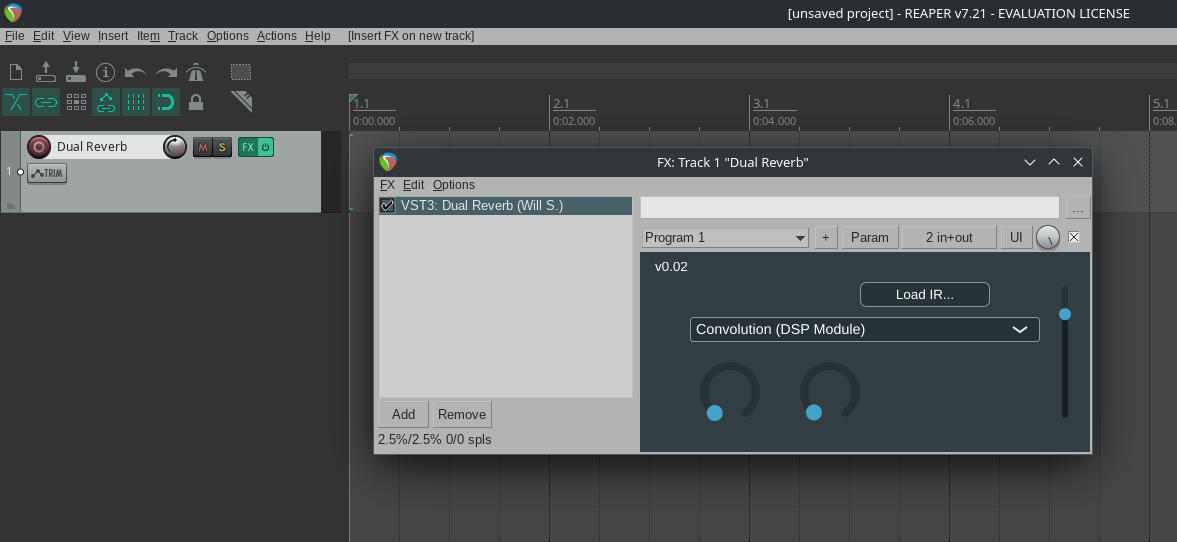
\includegraphics[width=14cm]{figures/DAW-1.png}
		}
		\caption{The reverb plugin running within Reaper.}
	\end{center}
\end{figure}

%%!TEX root = ../username.tex
\chapter{Musical Application}
\section{Selected Works}

%%!TEX root = ../username.tex
\chapter{Conclusion and Future Work}
\hspace*{-0.15cm}This barely scratches the surface. While the topics mentioned in this thesis cover the fundamentals of artificial reverberation, there are many different designs and improvements that can be made over the program as it is described here. Schroeder reverberators are considered a specific case to the more generalized structure known as a \textit{Feedback Delay Network (FDN)} \cite{schlecht2016lossless}. A modernized artificial reverberator will use this type of structure with a diffuser step, should one take the route of a purely artificial design. Through this design, a reverberator would split the audio into several channels - similar to that of Comb Filters in parallel - but would manipulate the signal by distributing the the amplitude amongst the matrix of channels to provide a more diffuse sound \cite{writeReverb}. This is just one area that is possible to improve upon.

Several improvements can be made during the prediction and measurement of Impulse Responses, as well. The Absorption Coefficients found in Table 5.1 were chosen as what best approximated the materials found in the room - a better selection of coefficients would likely yield a more accurate result. Along with this, the simplification of the room geomety would introduce some amount of error in the prediction as well - a better prediction would take each surface into account, including steps and curves of the performance walls. When recording, better practice would be to include a marker to better align the raw audio files with the impulse to deconvolve with - this is likely the culprit for the noise found in Figures 5.2 and 5.4.

The code itself can be improved upon, as well. In its current state, the Convolution approach includes several glitches in the audio output, which is likely due to the number of calculations required for the length of the Impulse Response. While building a ``Release'' build of the application \textit{significantly} improves the latency of this approach, it still can be improved upon with better tuning and usage of JUCE's DSP class. Similarly, the code behind the Schroeder Comb Filter approach can be improved through less copying of buffers - there is likely a more efficient solution that involves less usage of JUCE's classes that would allow for a larger number of filters in parallel before performance takes a hit, similar to what Freeverb was able to accomplish.

Despite this, this thesis provides a groundwork for any future audio engineer wishing to develop this type of application. I encourage anyone wishing to learn more to search and read through the citations used, as they contain a wealth of knowledge that this thesis only uses a fraction of. While the topics and filters used are specifically in the context of artificial reverberation, these same techniques can be applied to a wide variety of other effects, including distortion, vocoding, and autotune.

%\input{conclusion}

%%%%%%%%%%%%%%%%%%%%%%%%%%%%%%%%%%%%%%%%%%%%%%%%%%%%%%%
%
%  This section starts the back matter. The back matter includes appendices, indicies, and the
%  bibliography
%
%%%%%%%%%%%%%%%%%%%%%%%%%%%%%%%%%%%%%%%%%%%%%%%%%%%%%%%

\backmatter

%!TEX root = ../username.tex
\chapter*{Afterword}\label{after}
\addcontentsline{toc}{chapter}{Afterword}
\markboth{Afterword}{Afterword}
So how does a \lt session work? \lt loads the document class with any specified options and uses the information in the document class to decide on how the document will be formatted. At this point \lt loads any packages that the user has specified. Packages extend the basic \lt commands and formatting for special situations. \verb|woosterthesis| loads several packages by default and several others through class options; it is assumed you have these installed on your system. They are:
\ip{alltt},
\ip{amsfonts},
\ip{amsmath},
\ip{amssymb},
\ip{amsthm},
\ip{babel},
\ip{biblatex},
\ip{biblatex-chicago},
\ip{caption},
\ip{csquotes},
\ip{eso-pic},
\ip{eucal},
\ip{eufrak},
\ip{fancyhdr},
\ip{float},
\ip{floatflt},
\ip{fontenc},
\ip{fontspec},
\ip{geometry},
\ip{graphicx},
\ip{hyperref},
\ip{ifpdf},
\ip{ifthen},
\ip{ifxetex},
\ip{inputenc},
\ip{lettrine},
\ip{listings},
\ip{lmodern},
\ip{makeidx},
\ip{maple2e},
\ip{microtype},
\ip{pdftex},
\ip{polyglossia},
\ip{pxfonts},
\ip{setspace},
\ip{subfig},
\ip{textpos},
\ip{Ti\emph{k}Z},
\ip{verbatim},
\ip{wrapfig},
\ip{xcolor},
\ip{xltxtra},
and \ip{xunicode}.
The \texttt{woosterthesis} class assumes you are using pdf\TeX (support for postscript based TeX has been dropped as of 2006/17/11).

The \texttt{hyperref} package will make your thesis a linked document. \texttt{amsthm} is for altering the Theorem environments. \texttt{amsmath} implements almost all the mathematical symbols. \texttt{amssymb} adds the mathematical symbols not present in \texttt{amsmath}. \texttt{graphicx} and \texttt{eso-pic} are used to place graphics files in the thesis. \texttt{geometry} is used to set up the margins for the thesis. \texttt{setspace} is used to alter spacing by allowing a \texttt{singlespace}, \texttt{doublespace}, and \texttt{onehalfspace} environments. \texttt{biblatex} formats citations and references.  Documentation is included for some of the packages in the \verb|doc| folder.

These packages should all be installed with a full installation of TeXLive on OS X or Windows. On OS X one can use the the MacTeX installer as i-Installer is no longer supported as of 2007/1/1. On Windows one can use MikTeX to install all available packages which will install all the above. By default the MikTeX install does a minimal installation. You will need to run the updater to make your MikTeX installation aware of all the new packages.

There is also a new \TeX{} engine called \xt which allows one to use the native fonts on your system as text fonts in the document. More information can be found at the \href{http://scripts.sil.org/cms/scripts/page.php?site_id=nrsi&id=xetex}{\xt homepage}. If using \xt you will also need \ip{fontspec}, \ip{xunicode}, and \ip{xltxtra} which should be installed with \xt.

Once the packages are loaded, \lt begins to process the commands contained between the \texttt{document} tags. As it processes the commands, several auxiliary files are created. These files contain information needed for things like the Bibliography, Table of Contents, List of Figures, etc. We then process the file a second time to allow \lt to use its auxiliary files to fill in information. Some information may require three passes before it is displayed. Once \lt is done you are presented with a PDF of the output.

%%%%%%%%%%%%%%%%%%%%%%%%%%%%%%%%%%%%%%%%%%%%%%%%%%%%%%%
%
%  We used BibLaTeX and Biber to generate a Bibliography.
%
%%%%%%%%%%%%%%%%%%%%%%%%%%%%%%%%%%%%%%%%%%%%%%%%%%%%%%%

%\nocite{*} % This command forces all the bibliography references to be printed -- not just
              % those that were explicitly cited in the text.  If you comment this out, the bibliography
              % will only include cited references.
\printbibliography[title=References,heading=bibintoc]% load our Bibliography file

%%%%%%%%%%%%%%%%%%%%%%%%%%%%%%%%%%%%%%%%%%%%%%%%%%%%%%%
%
%                                                                Index
%
%  Uncomment the lines below to include an index. To get an index you must put 
%  \index{index text} after any words that you want to appear in the index.
%  Subentries are entered as \index{index text!subentry text}. You must also run the
%  makeindex program to generate the index files that LaTeX uses. The PCs are set to run
%  makeindex automatically.
%
%%%%%%%%%%%%%%%%%%%%%%%%%%%%%%%%%%%%%%%%%%%%%%%%%%%%%%%

\ifthenelse{\boolean{index}}{
\cleardoublepage
\phantomsection
\addcontentsline{toc}{chapter}{Index}
\printindex}{}

%%%%%%%%%%%%%%%%%%%%%%%%%%%%%%%%%%%%%%%%%%%%%%%%%%%%%%%
%
%                                                                Colophon
%
%  A Colophon is a section of a printed document that acknowledges the designers and printers of the work.
% The colophon also includes information about the fonts and paper used in the printing. It is not required 
% for your IS and can be commented out.
%
%%%%%%%%%%%%%%%%%%%%%%%%%%%%%%%%%%%%%%%%%%%%%%%%%%%%%%%

\ifthenelse{\boolean{colophon}}{
\begin{colophon}
This Independent Study was designed by Dr. Jon Breitenbucher.\newline
It was edited and set into type in Wooster, Ohio,\newline
using the \ifthenelse{\boolean{xetex}}{\XeTeX\ typesetting system designed by Jonathan Kew}{\LaTeX\ typesetting system designed by Leslie Lamport}\newline
and based on the original \TeX\ system of Donald Knuth.\newline
It was printed and bound by Office Services at The College of Wooster.

The text face is Adobe Garamond Pro, designed by Robert Slimbach.\newline
This is the Opentype version distributed by Adobe Systems\newline
and purchased as part of the Adobe Type Classics for Learning.

The paper is standard laser copier paper and not of archival quality.
\end{colophon}}{}
\clearpage\thispagestyle{empty}\null\clearpage
\end{document}
